\section{Perspective Projection}

\begin{figureBox}[label={fig:ortho-vs-persp}, width=0.8\linewidth]{Orthographic and perspective projections}
    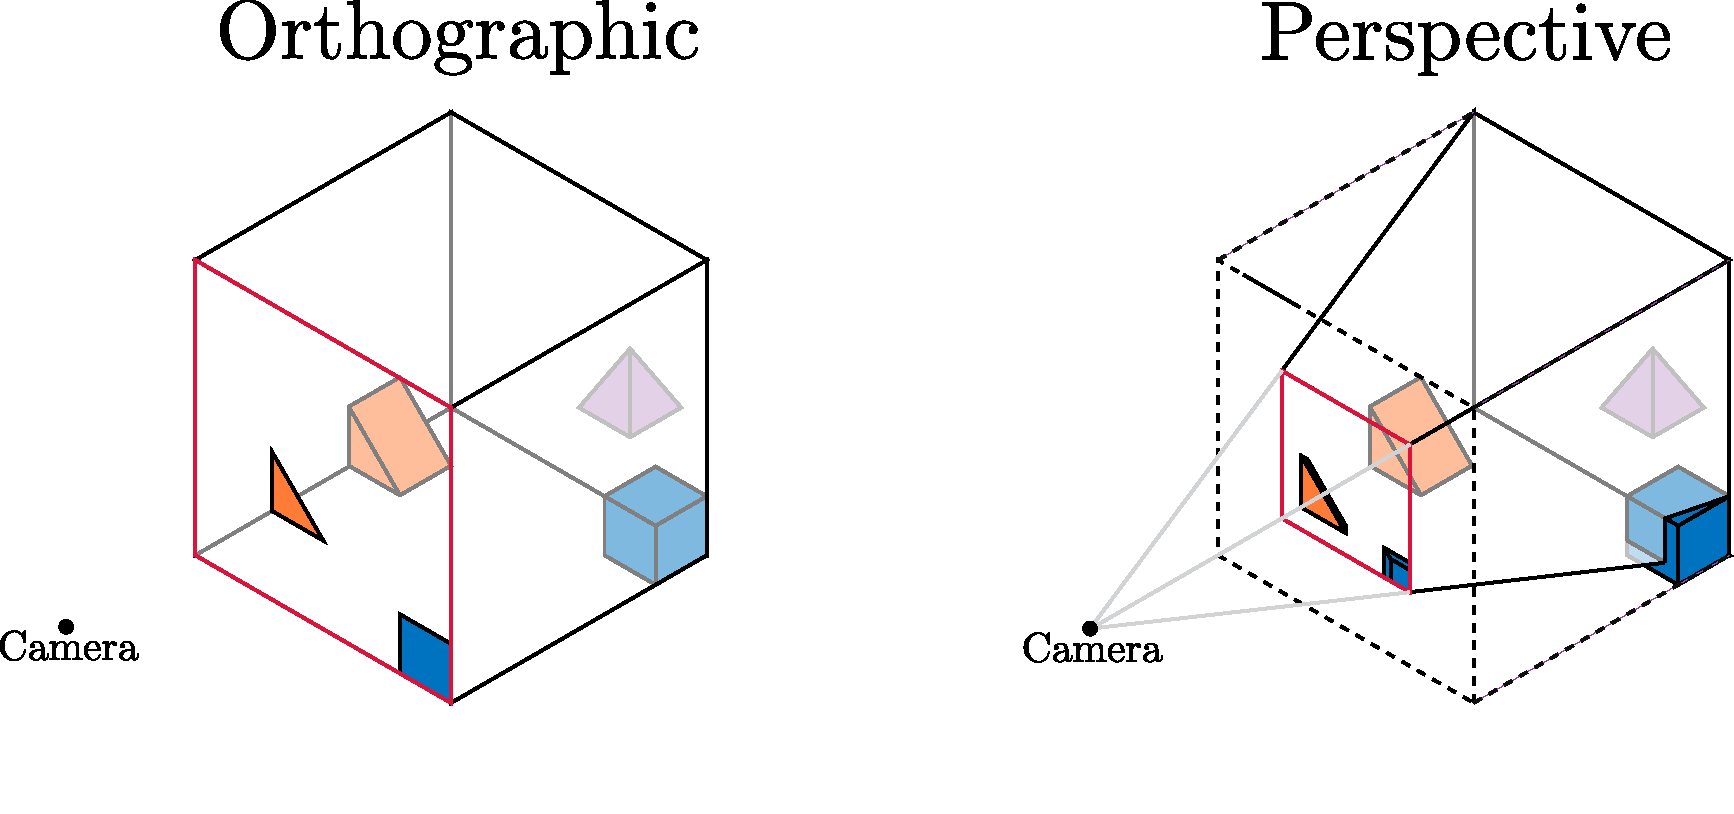
\includegraphics[width = 0.8\linewidth]{./background/figures/projection/ortho-vs-persp.pdf}
\end{figureBox}

To represent 3D space on a 2D surface OpenGL supports two types of projections: perspective and orthographic as seen in Fig~\ref{fig:ortho-vs-persp}. Orthographic features parallel projection lines (orthogonal to the projection plane), which means that it does not depict the effect of perspective. Distances are preserved, making it useful for technical drawings where measurements need to be precise and not skewed by perspective (For example all diagrams in this report are from the orthographic perspective). Unlike orthographic projections, perspective projections simulate the way the human eye perceives the world, with objects appearing smaller the further away they are from the viewpoint as the projection lines converge at a vanishing point on the horizon. If we wish to create the illusion of volumetric display in this project we must use a perspective projection. \\

\begin{figureBox}[label={fig:persp-projection}, width=0.8\linewidth]{Using frustum to generate a perspective projection}
    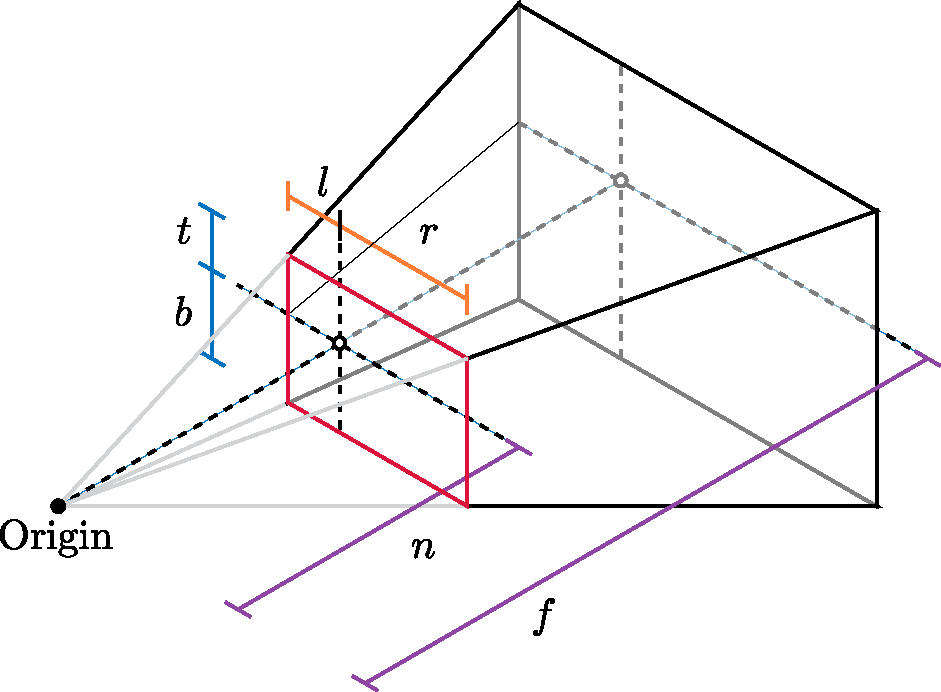
\includegraphics[width = 0.8\linewidth]{./background/figures/projection/persp-projection.pdf}
\end{figureBox}

OpenGL provides the \texttt{frustum} function as seen in Fig~\ref{fig:persp-projection} which can be used to construct the perspective matrix (it is worth noting that OpenGL uses homogeneous coordinates so the matrix is 4x4):     
\[
    \begin{bmatrix}
        \frac{2n}{r-l} & 0              & \frac{r+l}{r-l}  & 0                \\
        0              & \frac{2n}{t-b} & \frac{t+b}{t-b}  & 0                \\
        0              & 0              & -\frac{f+n}{f-n} & -\frac{2fn}{f-n} \\
        0              & 0              & -1               & 0                \\
    \end{bmatrix}
\] 
This maps a specified viewing frustum to screen space (with intermediate steps handled by OpenGL) \cite{hearn2004computer}. This viewing frustum is specified by six parameters: $l$, $r$, $b$, $t$, $n$ and $f$ which represent the left, right, bottom, top, near, and far extents of the frustum. These parameters define the sides of the near-clipping plane, highlighted in red, relative to the origin of the coordinate system. These parameters do not represent distances or magnitudes in a traditional sense but rather define the vectors from the center of the near-clipping plane to its edges. \\


The $l$ and $r$ parameters specify the horizontal boundaries of the frustum on the near-clipping plane, with the left typically being negative and the right positive, defining the extent to which the frustum extends to the left and right of the origin. Similarly, the $b$ and $t$ parameters determine the vertical boundaries, with the bottom often negative and the top positive, expressing the extent of the frustum below and above the origin. \\

The $n$ and $f$ parameters are scalar values that specify the distances from the origin to the near and far clipping planes along the view direction. Altering the value of $n$ will change the angles of the lines that connect the corners of the near plane to the eye, effectively changing the "field of view". Changing the value $f$ affects the range of depth that is captured within the scene but not the view. \\

If we can track the position of a viewer's eye in real time then we can create the illusion of a 3D scene behind and in front of a display using this \texttt{frustum} function. This can be done fairly trivially following Robert Kooima's method he sets out in "Generalized Perspective Projection" to calculate $f$, $l$, $r$, $b$, $t$, $n$ as the viewer's eye changes position \cite{kooima2009generalized}. 

\subsection{Generating the perspective projection}

The first step we must take is to record the position of the screen we are projecting onto in 3D space relative to the coordinate system of the tracking device, "tracker-space". To encode the position and size of the screen we take 3 points, $p_a$, $p_b$ and $p_c$ which represent the lower-left, lower-right and upper-left points of the screen respectively when viewed from the front on. These points can be used to generate an orthonormal basis for the screen comprised of $s_r$, $s_u$ and $s_n$ which represents the directions up, right and normal to the screen respectively as seen in Fig~\ref{fig:perspective-screen}. We can compute these values from the screen corners as follows:
\[s_r = \frac{p_b-p_a}{||p_b-p_a||} \quad s_u = \frac{p_c-p_a}{||p_c-p_a||} \quad s_n = \frac{s_r\times s_u}{||s_r \times s_u||}\]

\begin{figureBox}[label={fig:perspective-screen}, width=0.8\linewidth]{Defining a screen in 3D space}
    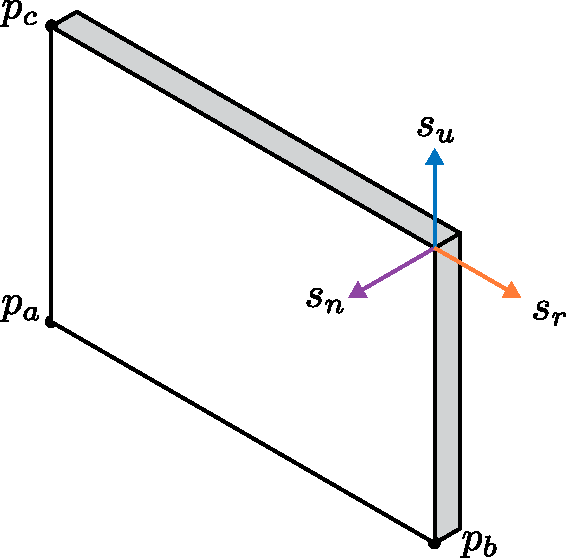
\includegraphics[width = 0.3\linewidth]{./background/figures/projection/screen.pdf}
\end{figureBox}

Next, we introduce the viewer's eye which we will refer to as $p_e$. We can draw 2 vectors $v_b$, $v_c$ from the viewer's eye $p_e$ to the corners of the screen $p_b$, $p_c$ as seen in Fig~\ref{fig:screen-extents}. In the diagram, we also have labeled the components of each of these vectors in the basis of the screen. We can compute these as follows:
\[ v_a = p_a - p_e \quad v_b = p_b - p_e \quad v_c = p_c - p_e\] 

To calculate the required values for our \texttt{frustum} OpenGL function we must first find the point where a line drawn perpendicular to the plane of the screen that passes through $p_e$ strikes the screen. We refer to this point as the {\it screen-space-origin}, it is worth noting that this point can lie outside the screen (the rectangle bounded by $p_a$, $p_b$, $p_c$). We can find the distance of the {\it screen-space-origin} from the eye $p_e$ by taking the component of the screen basis vector $s_n$ in either of the vectors $v_b$ and $v_c$. However, as $s_n$ is in the opposite direction we must invert the result. Similarly, we can calculate $t$ by taking the component of $v_c$ in the basis vector $s_u$, $b$ by $v_b$ in $s_u$, $l$ by $v_c$ in $s_r$ and lastly $r$ by $v_b$ in $s_r$. We can compute these as follows:
\[ d= -(s_n \cdot v_a) \quad l = (v_c \cdot s_r) \quad r = (v_b \cdot s_r) \quad b = (v_b \cdot s_u) \quad t = (v_c \cdot s_u) \]

\begin{figureBox}[label={fig:screen-extents}, width=0.8\linewidth]{Screen Intersection with view}
    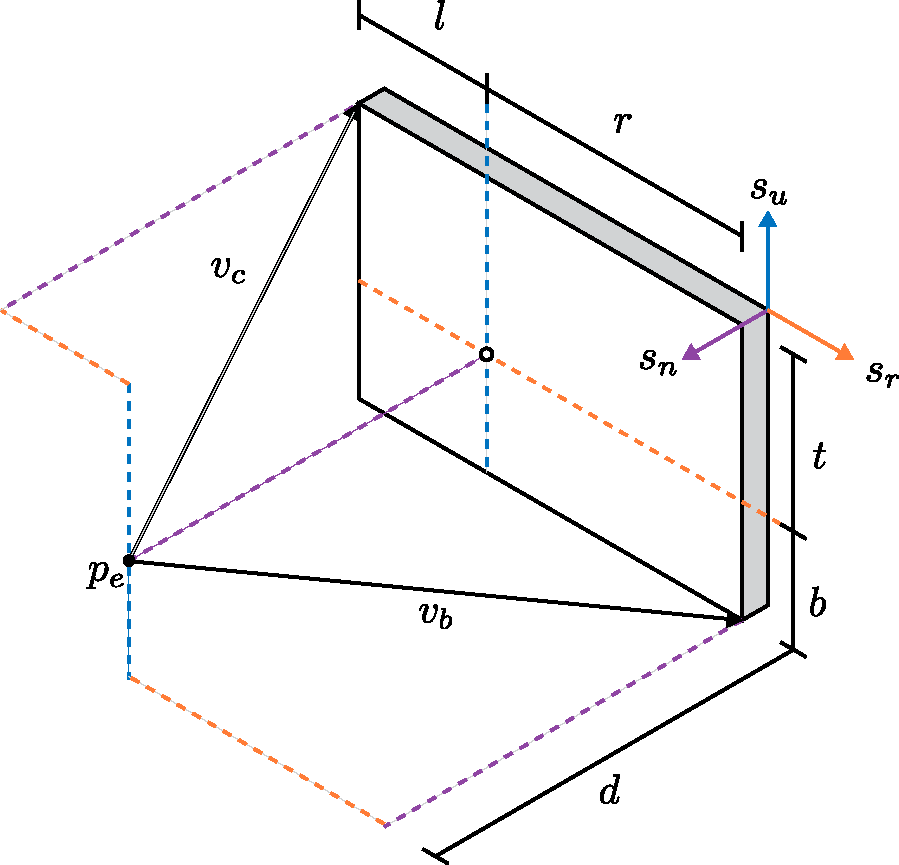
\includegraphics[width = 0.5\linewidth]{./background/figures/projection/eye-projection.pdf}
\end{figureBox}

We can now generate a projection matrix by calling \texttt{frustum} using $d$ as our near-clipping plane distance $n$ with an arbitrary value for the far-clipping plane $f$ depending on our required scene depth. We have now successfully generated our viewing frustum but we still have a few issues. Firstly our frustum has been defined in tracker space so it is aligned with the direction of our camera not the normal of our screen. We can remedy this by applying a rotation matrix M to align our frustum with $s_n$, $s_u$ and $s_r$, the basis of our screen as seen in Fig~\ref{fig:basis-change}. M is defined as follows:
\[
    \begin{bmatrix}
        v_{rx} & v_{ry} & v_{rz} & 0 \\
        v_{ux} & v_{uy} & v_{uz} & 0 \\
        v_{nx} & v_{ny} & v_{nz} & 0 \\
        0      & 0      & 0      & 1 \\
    \end{bmatrix}
\]

\begin{figureBox}[label={fig:basis-change}, width=0.8\linewidth]{Rotating the frustum from tracker space alignment into screen space alignment}
    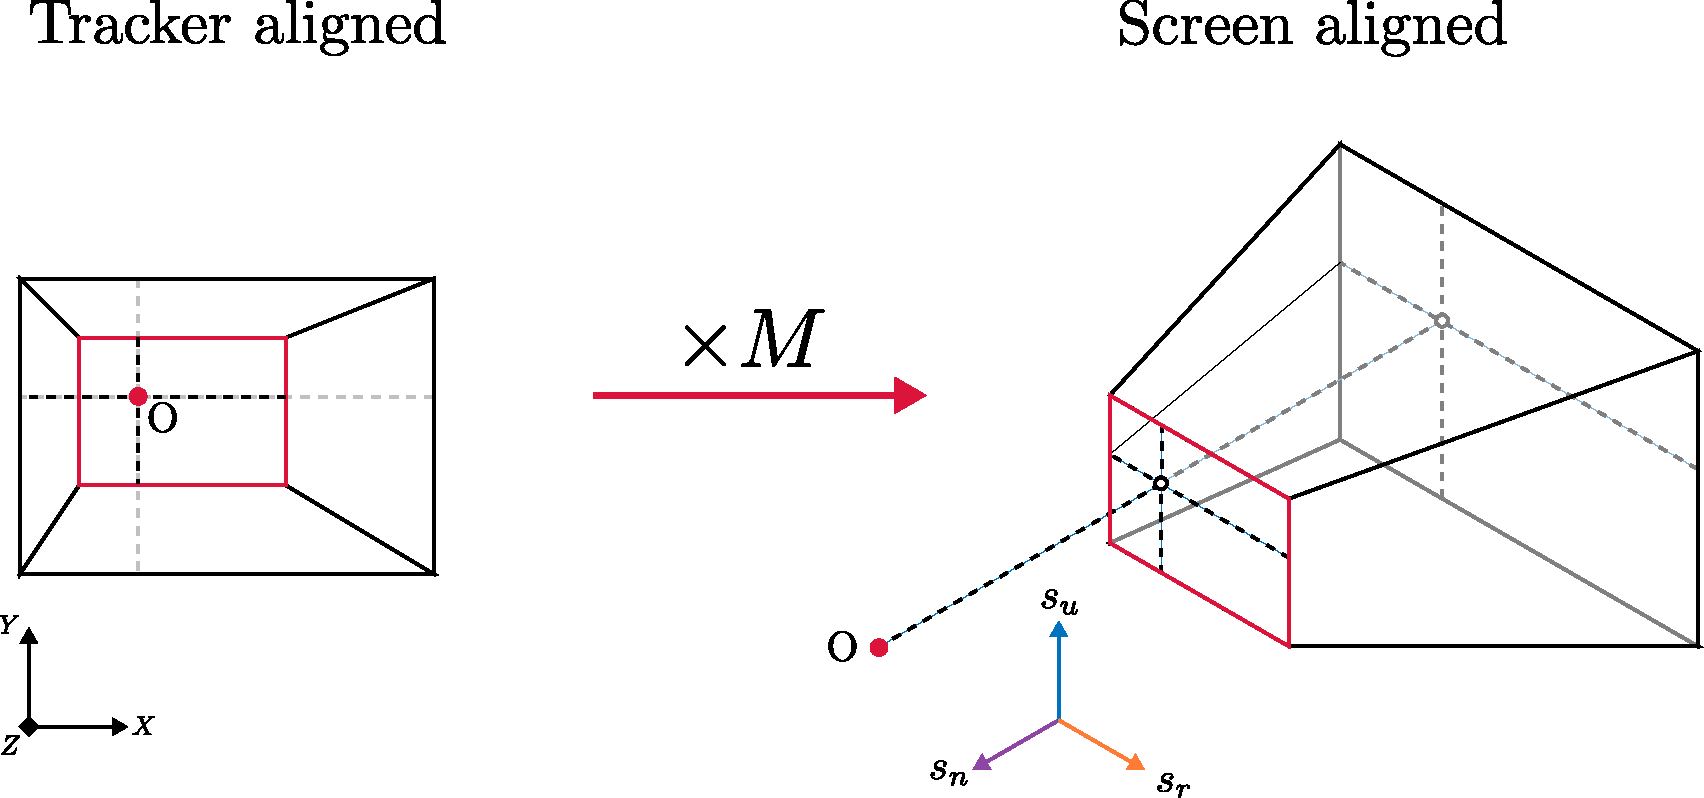
\includegraphics[width = 0.8\linewidth]{./background/figures/projection/realignment.pdf}
\end{figureBox}

The second problem we have is that we want our projection matrix to move around with the viewer's eye however the mathematics of perspective projection disallow this, with the camera assumed to be at the origin. To translate our viewing frustum to our eye position we must instead translate our eye position (and the whole world) to the origin of our frustum. This can be done with a translation matrix $T$ as seen in Fig~\ref{fig:frust-translation}. $T$ can be generated with the OpenGL function \texttt{translate} where we want to offset it by the vector from our Origin to the viewer's eye $p_e$. T is defined as follows:
\[
    \begin{bmatrix}
        1 & 0 & 0 & -p_{ex} \\
        0 & 1 & 0 & -p_{ey} \\
        0 & 0 & 1 & -p_{ez} \\
        0 & 0 & 0 & 1       \\
    \end{bmatrix}
\]

\begin{figureBox}[label={fig:frust-translation}, width=0.8\linewidth]{Translating the viewing frustum to sit inside the screen}
    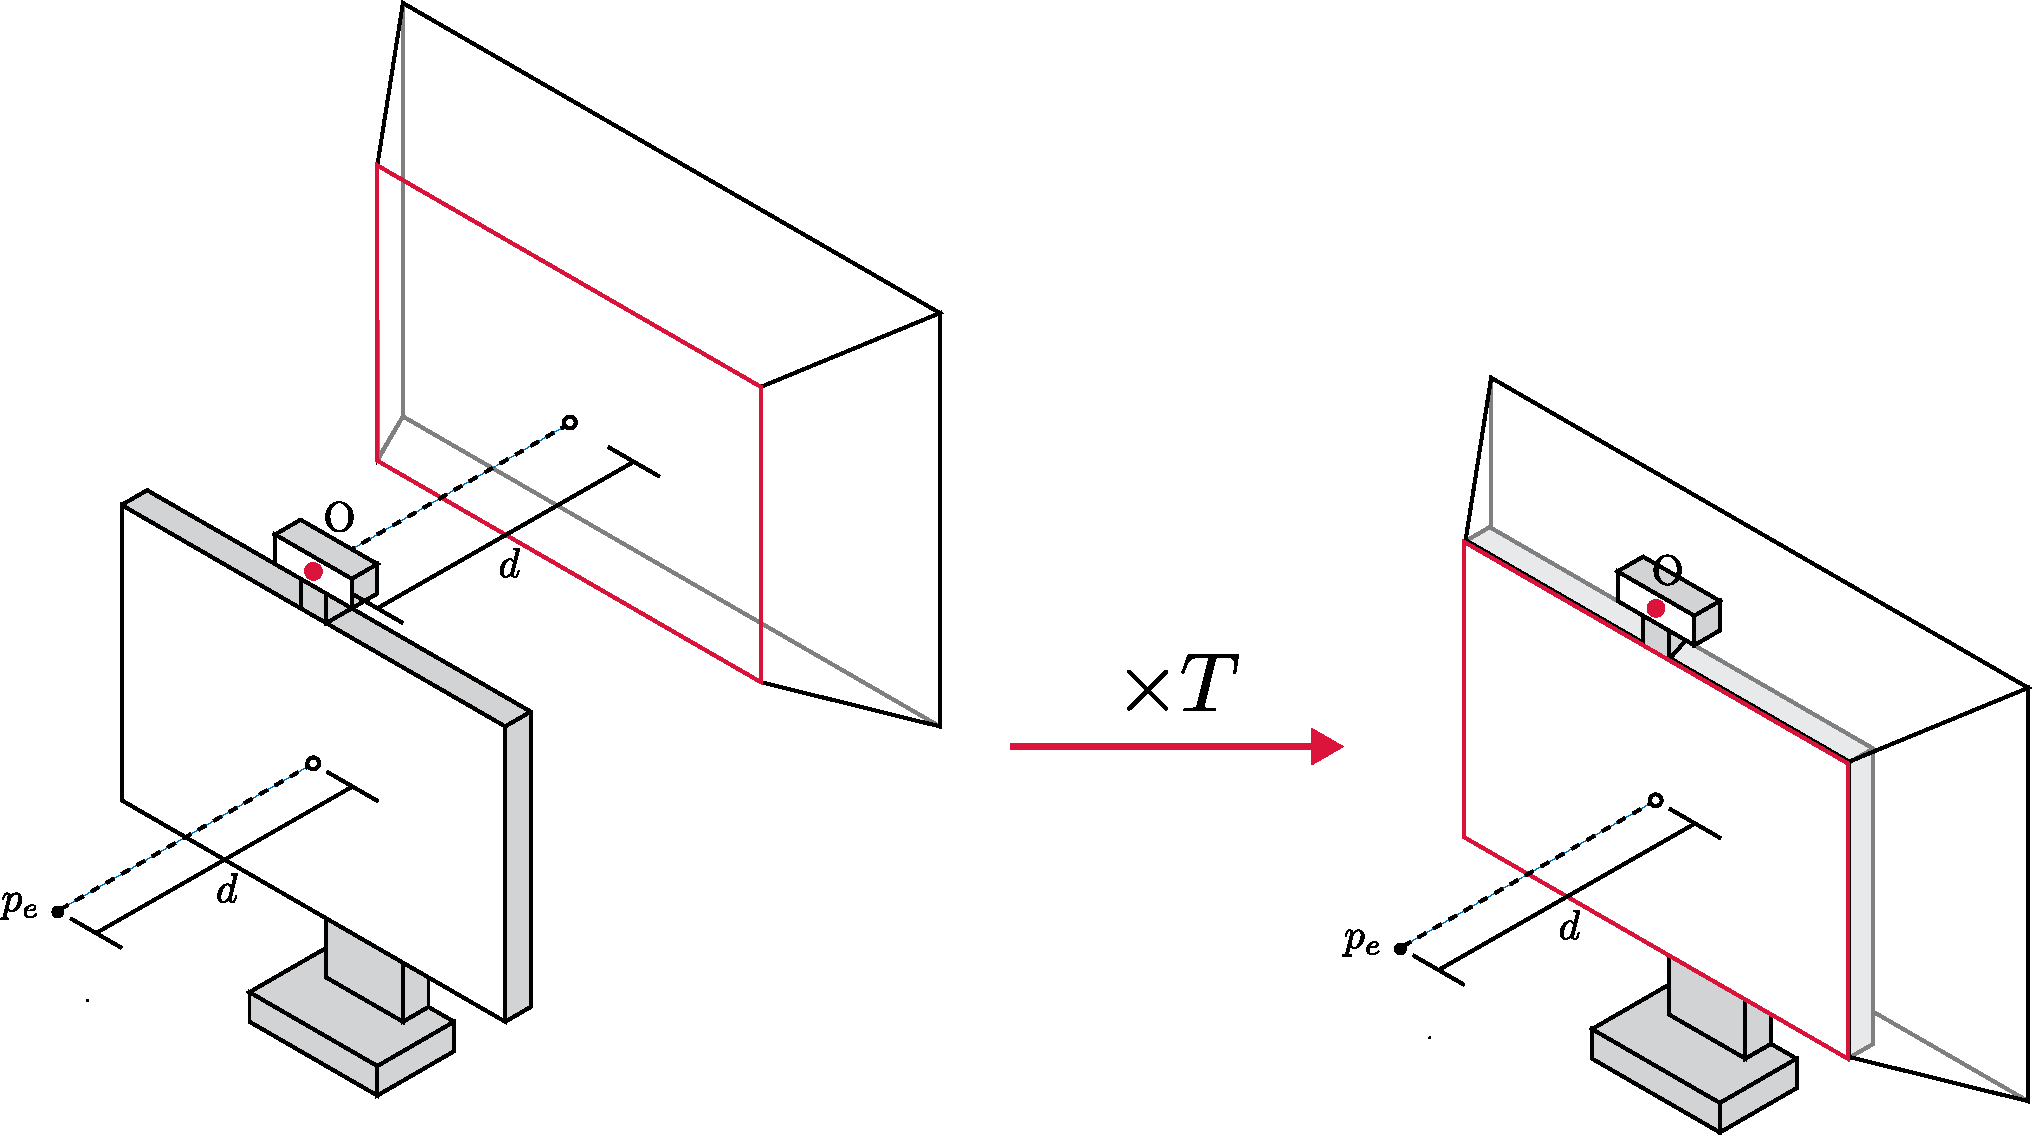
\includegraphics[width = 0.8\linewidth]{./background/figures/projection/frust-translation.pdf}
\end{figureBox}

We now have a working method for projecting virtual objects behind our screen onto our screen however it is also possible if we desire to project objects in front of our screen onto the screen as well as long as they lie within the pyramid formed between the edges of the screen and the viewer's eye. We can scale the near-clipping plane from the plane of the screen to a small distance $n$ from our eye as seen in Fig~\ref{fig:extending-near} giving us scaled-down values of $t$, $b$ $l$ and $r$ we can use for our new viewing frustum which we call $t_n$, $b_n$ $l_n$ and $r_n$. They are defined as follows:
\[
    l_n = (v_c \cdot s_r) \frac{n}{d} \quad r_n = (v_b \cdot s_r) \frac{n}{d} \quad b_n = (v_c \cdot s_u) \frac{n}{d} \quad t_n = (v_b \cdot s_u) \frac{n}{d}
\]

So our final viewing frustum takes in the frustum extents $t_n$, $b_n$ $l_n$ and $r_n$ and $n$ and $f$ defining the distances to the near and far clipping plane.
\begin{figureBox}[label={fig:extending-near}, width=0.8\linewidth]{Extending the near plane to not clip out objects in front of the screen}
    \centering
    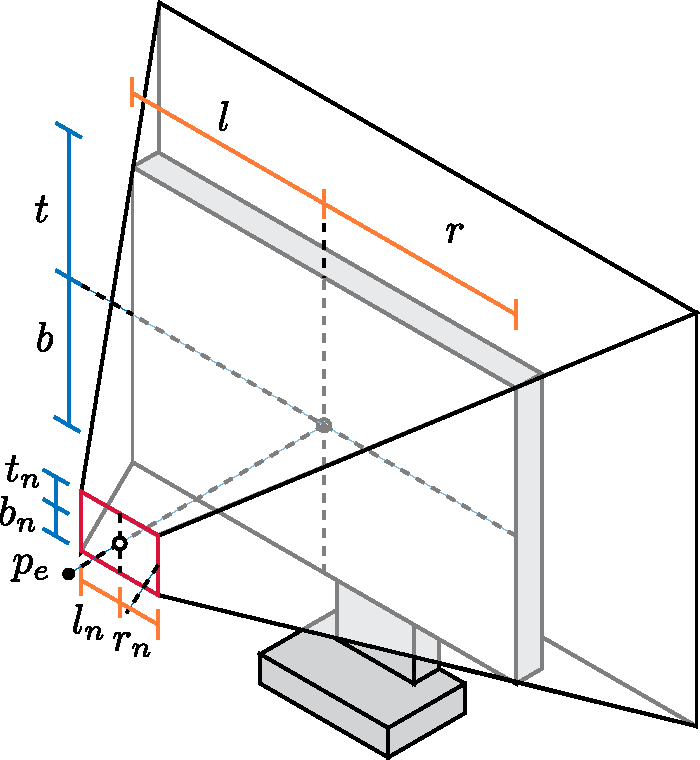
\includegraphics[width = 0.5\linewidth]{./background/figures/projection/extending-near.pdf}
\end{figureBox}

Following these steps, we can create an accurate projection providing the perspective we would expect to see if there was a scene in front and behind our screen. 

\subsection{Sample code}
Below in Listing~\ref{fig:c-projection} we have given an example of a function implementing the process we have just described in C++.

\codeBoxFile[label={fig:c-projection}]{cpp}{./background/code/projection.cpp}{projection.cpp, Sample code for creating the 3D illusion projection}
